% Select language used in document (ngerman or english). Automatically
% generated text is translated accordingly.
% use \selectthesislanguage in body.tex to switch to default language

%\documentclass[english, paper]{mmt} % use for BA1
\documentclass[english, bachelorthesis]{mmt} % use for BA2
%\documentclass[ngerman, masterthesis]{mmt} % use for Master thesis

\usepackage{mathptmx}
\usepackage{graphicx}
\usepackage{times}
\usepackage{subfig}
\usepackage{float}
\usepackage[utf8]{inputenc}
\usepackage{listings}
\usepackage{makecell}
\usepackage[toc,page]{appendix}
\usepackage{hyperref}
\hypersetup{
    colorlinks,
    citecolor=black,
    filecolor=black,
    linkcolor=black,
    urlcolor=black
}
\usepackage{breakurl}

\usepackage{amsmath}
\usepackage[autostyle,german=guillemets]{csquotes}

% moved to cls file. use \selectthesislanguage to switch to default language
%\usepackage[english,ngerman]{babel}

\usepackage{abbrevs}
%% the following solves a bug in the abbrevs package, that adds an empty
%% space after the abbrev
\makeatletter
\renewcommand\maybe@space@{%
  % \@tempswatrue % <= this is in the original
  \maybe@ictrue % <= this is new
  \expandafter   \@tfor
    \expandafter \reserved@a
    \expandafter :%
    \expandafter =%
                 \nospacelist
                 \do \t@st@ic
  % \if@tempswa % <= this is in the original
  \ifmaybe@ic % <= this is new
    \space
  \fi
}
\makeatother
%%


\usepackage{listings}
\usepackage{color}
\definecolor{lightgray}{rgb}{.9,.9,.9}
\definecolor{darkgray}{rgb}{.4,.4,.4}
\definecolor{purple}{rgb}{0.65, 0.12, 0.82}
\lstdefinelanguage{JavaScript}{
  keywords={break, case, catch, continue, debugger, default, delete, do, else, false, finally, for, function, if, in, instanceof, new, null, return, switch, this, throw, true, try, typeof, var, let, const, void, while, with},
  morecomment=[l]{//},
  morecomment=[s]{/*}{*/},
  morestring=[b]',
  morestring=[b]",
  ndkeywords={class, export, boolean, throw, implements, import, this},
  keywordstyle=\color{blue}\bfseries,
  ndkeywordstyle=\color{darkgray}\bfseries,
  identifierstyle=\color{black},
  commentstyle=\color{purple}\ttfamily,
  stringstyle=\color{red}\ttfamily,
  sensitive=true
}

\lstset{
   language=JavaScript,
   backgroundcolor=\color{lightgray},
   extendedchars=true,
   basicstyle=\footnotesize\ttfamily,
   showstringspaces=false,
   showspaces=false,
   numbers=left,
   numberstyle=\footnotesize,
   numbersep=9pt,
   tabsize=2,
   breaklines=true,
   showtabs=false,
   captionpos=b
}

\usepackage[authordate,bibencoding=auto,strict,noibid,backend=biber]{biblatex-chicago}
\bibliography{bibliography}

%% Add configuration options
\newabbrev{\authorname}{Isabella Sperr}
\newabbrev{\authormail}{isperr.mmt-b2016@fh-salzburg.ac.at}
\newabbrev{\titlename}{Designing interfaces about health literacy that are particularly suited for children and their abilities}
\newabbrev{\advisor}{FH-Prof. DI Dr. Simon Ginzinger}
%\newabbrev{\secondadvisor}{Titel Vorname Nachname}
\newabbrev{\thesisdate}{12.08.2019}
\newabbrev{\keywordsenglish}{word1, word2, word3}
\newabbrev{\keywordsgerman}{wort1, wort2, wort3}


%% Paper title.

\title{\titlename}

%% This is how authors are specified in the conference style

%% Author 
\author{ \authorname\\ \scriptsize \authormail \\ \scriptsize 
\ifmmtlanguagegerman FH Salzburg \else Salzburg University of Applied Sciences \fi
}

%% A teaser figure can be included as follows, but is not recommended since
%% the space is now taken up by a full width abstract.
%\teaser{
%  \includegraphics[width=1.5in]{sample.eps}
%  \caption{This can be a teaser image of the thesis.}
%}

%% Abstract section for paper format.
\abstract{
    \ifmmtlanguagegerman 
        \selectlanguage{ngerman}
        Lorem ipsum dolor sit amet, consectetur adipiscing elit. Aenean venenatis nulla vestibulum dignissim molestie. Quisque tristique tortor vitae condimentum egestas. Donec vitae odio et quam porta iaculis ut non metus. Sed fermentum mauris non viverra pretium. Nullam id facilisis purus, et aliquet sapien. Pellentesque eros ex, faucibus non finibus a, pellentesque eu nibh. Aenean odio lacus, fermentum eu leo in, dapibus varius dolor. Lorem ipsum dolor sit amet, consectetur adipiscing elit. Proin sit amet ornare velit. Donec sit amet odio eu leo viverra blandit. Ut feugiat justo eget sapien porttitor, sit amet venenatis lacus auctor. Curabitur interdum ligula nec metus sollicitudin vestibulum. Fusce placerat augue eu orci maximus, id interdum tortor efficitur.
    \else 
        \selectlanguage{english}
        This thesis aims to disclose necessary features that need to be included in an interface about health literacy that is particularly suitable for children. 
As \textcite{walker2000screen, sharmin2012effect} mention in their papers, technology has gone through great developmental stages and has improved a lot over the last 20 years. As a consequence, technology has become a part of our everyday lives \autocite{gikas2013mobile, gossen2012search}. As \textcite{walker2000screen} mention in their paper, it is not surprising that schools too hope to use technology for educational purposes.  
Thus, in the course of this study, a prototype in the form a quiz was designed. Since the appearance was not the only thing that had to be adapted to the needs and abilities of children, appropriate content had to be chosen too. As a result, the content of the prototype is health literacy with a focus on nutrition. As the study of \textcite{jordan2015gesundheitskompetenz} showed, sometimes even adults are not informed sufficiently. Therefore, it is essential to teach children about health literacy as soon as possible.\\
The developed prototype and the associated testing have revealed that children prefer engaging and rather gamified applications. Furthermore, the majority of the tested children are adequately informed about proper nutrition.
    \fi
}

%%%%%%%%%%%%%%%%%%%%%%%%%%%%%%%%%%%%%%%%%%%%%%%%%%%%%%%%%%%%%%%%
%%%%%%%%%%%%%%%%%%%%%% START OF THE PAPER %%%%%%%%%%%%%%%%%%%%%%
%%%%%%%%%%%%%%%%%%%%%%%%%%%%%%%%%%%%%%%%%%%%%%%%%%%%%%%%%%%%%%%%%

\begin{document}
% TODO switch for english, german
\selectthesislanguage

\pagenumbering{gobble}

 % group open
\ifmmtpaper 
\begingroup 
    % is required because paper template messes with sizes
    \fontsize{12}{18}\selectfont        
    \setlength{\parindent}{0pt}
    \setlength{\parskip}{5pt plus 2pt minus 1pt}
    \sectionfont{\fontsize{14}{15}\selectfont}
\fi

    \begin{titlepage}

% check if second advisor exists
\newcommand{\printsecondadvisor}[1]{%
  \ifcsname#1\endcsname%
  \ifmmtlanguagegerman ZweitbetreuerIn: \else Second Advisor: \fi \secondadvisor 
  \else%
    
  \fi%
}

\ifmmtmasterthesis

    
    % \begin{center}
    %     \Huge{ 
    %     	\textbf{\ifmmtlanguagegerman Masterarbeit \else Master Thesis \fi}
    %     }
    % \end{center}
    
    \newpage
    
    \thispagestyle{empty}
    
    \hfill 
\includegraphics[height=1.5cm]{images/FHSLogo.jpg}
    
    \vspace*{2cm}
    
    \Large{
    \titlename
    
    \vspace*{1cm}
    
    \ifmmtlanguagegerman
    Masterarbeit zur Erlangung des akademischen Grades
    \else
    Master thesis in partial fulfilment of the requirements for\\ the degree of 
    \fi
    
    \vspace*{0.5cm}
    
    \textit{Master of Science}
    }
    
    
    \vspace*{1.5cm}
    {\large
    \ifmmtlanguagegerman AutorIn: \else Author: \fi \authorname
    }
    \vfill
    
    {\normalsize
    \ifmmtlanguagegerman
    Vorgelegt am FH-Masterstudiengang MultiMediaTechnology, Fachhochschule Salzburg
    \else
    Submitted to the Master degree program MultiMediaTechnology, Salzburg University of Applied Sciences
    \fi
    
    
    \vspace*{1cm}
    
    \ifmmtlanguagegerman BetreuerIn: \else Advisor: \fi
    \advisor
    \\    
    \printsecondadvisor{secondadvisor}
    
    \vfill
    
    Salzburg, \ifmmtlanguagegerman Österreich, \else Austria, \fi  \thesisdate
    }

\else % Bachelor thesis title page

    \begin{center}
    
    
\includegraphics[width=5cm]{images/FHSLogo.jpg}


    \vspace*{4cm}
    
    \fontsize{20.79}{18pt}{\selectfont        
    %\Large{
    	\textit{\textbf{\titlename}}
    %}
    }
    
    \vspace*{4cm}
    
    \fontsize{20.79}{18pt}{%\large{
    \ifmmtlanguagegerman
    	\textbf{Bachelorarbeit \ifmmtpaper 1 \else 2 \fi }
    \else
        \textbf{Bachelor Thesis \ifmmtpaper 1 \else 2 \fi }
    \fi
    }
    
    
    \end{center}
    
    \vfill
    
    %\begin{tabular}{ll}
    \ifmmtlanguagegerman AutorIn: \else Author: \fi  \authorname  \\
    \ifmmtlanguagegerman BetreuerIn: \else Advisor: \fi \advisor \\
    \printsecondadvisor{secondadvisor}
    
    Salzburg, \ifmmtlanguagegerman Österreich, \else Austria, \fi \thesisdate
    
    
    
    % uncomment the following 3 lines for an optional lock flag, max. 2 years!
    %\hfill
    %\color{red}
    %\framebox{Sperrvermerk bis 20/01/2012}

\fi

\end{titlepage}
        
    \onecolumn           
    
    \pagenumbering{roman}
    
    \newpage
    
\ifmmtlanguagegerman
\subsection*{Eidesstattliche Erklärung}


Ich erkläre hiermit eidesstattlich, dass  ich  die vorliegende Arbeit selbständig  und ohne fremde Hilfe verfasst, und keine  anderen  als die angegeben Quellen und  Hilfsmittel benutzt  habe. Weiter versichere ich hiermit, dass ich   die den benutzten Quellen  wörtlich oder inhaltlich entnommenen Stellen als solche kenntlich gemacht habe.

Die Arbeit wurde bisher in gleicher oder ähnlicher Form keiner anderen Prüfungskommission weder im In- noch im Ausland vorgelegt und auch nicht veröffentlicht.

\else

\subsection*{Affidavit}

I herewith declare on oath that I wrote the present thesis without the help of third persons and without using any other sources and means listed herein; I further declare that I observed the guidelines for scientific work in the quotation of all unprinted sources, printed literature and phrases and concepts taken either word for word or according to meaning from the Internet and that I referenced all sources accordingly.

This thesis has not been submitted as an exam paper of identical or similar form, either in Austria or abroad and corresponds to the paper graded by the assessors.

\fi

\vspace*{3cm}

%{\bf \thesisdate{}}


\hfill

\ifmmtlanguagegerman
$\overline{Datum \hspace{2cm}}$ \hfill $\overline{{Unterschrift}\hspace{3cm}}$

\vspace*{1cm}

\hfill $\overline{{Vorname\hspace{2cm}Nachname}}$
 
 \else
 $\overline{Date \hspace{2cm}}$ \hfill $\overline{{Signature}\hspace{4cm}}$

\vspace*{1cm}

 \hfill $\overline{{First~Name\hspace{2cm}Last~Name}}$
 \fi

  % comment out for expose

% group closing
\ifmmtpaper
\endgroup
\fi

%\ifmmtpaper\else
    
    \newpage
    \selectlanguage{ngerman}
    \section*{Kurzfassung}
    Lorem ipsum dolor sit amet, consectetur adipiscing elit. Aenean venenatis nulla vestibulum dignissim molestie. Quisque tristique tortor vitae condimentum egestas. Donec vitae odio et quam porta iaculis ut non metus. Sed fermentum mauris non viverra pretium. Nullam id facilisis purus, et aliquet sapien. Pellentesque eros ex, faucibus non finibus a, pellentesque eu nibh. Aenean odio lacus, fermentum eu leo in, dapibus varius dolor. Lorem ipsum dolor sit amet, consectetur adipiscing elit. Proin sit amet ornare velit. Donec sit amet odio eu leo viverra blandit. Ut feugiat justo eget sapien porttitor, sit amet venenatis lacus auctor. Curabitur interdum ligula nec metus sollicitudin vestibulum. Fusce placerat augue eu orci maximus, id interdum tortor efficitur.
    \ifmmtmasterthesis
    
    \vspace*{0.5cm} 
    \textbf{Schlüsselwörter:~} \keywordsgerman
    \fi
    \newpage
    \selectlanguage{english}
    \section*{Abstract}
    This thesis aims to disclose necessary features that need to be included in an interface about health literacy that is particularly suitable for children. 
As \textcite{walker2000screen, sharmin2012effect} mention in their papers, technology has gone through great developmental stages and has improved a lot over the last 20 years. As a consequence, technology has become a part of our everyday lives \autocite{gikas2013mobile, gossen2012search}. As \textcite{walker2000screen} mention in their paper, it is not surprising that schools too hope to use technology for educational purposes.  
Thus, in the course of this study, a prototype in the form a quiz was designed. Since the appearance was not the only thing that had to be adapted to the needs and abilities of children, appropriate content had to be chosen too. As a result, the content of the prototype is health literacy with a focus on nutrition. As the study of \textcite{jordan2015gesundheitskompetenz} showed, sometimes even adults are not informed sufficiently. Therefore, it is essential to teach children about health literacy as soon as possible.\\
The developed prototype and the associated testing have revealed that children prefer engaging and rather gamified applications. Furthermore, the majority of the tested children are adequately informed about proper nutrition.
    \ifmmtmasterthesis
        
    \vspace*{0.5cm} 
    \textbf{Keywords:~} \keywordsenglish
    \fi
    \selectthesislanguage
    
    \newpage
    \tableofcontents
    
    \newpage
    \ifmmtlanguagegerman
\section*{Abkürzungsverzeichnis}
\else
\section*{Abbreviations}
\fi

\begin{table}[h]		
	\begin{tabular}{ll}
		AR & Augmented Reality 
	\end{tabular}
\end{table}
    \listoffigures
    \lstlistoflistings
    \listoftables
    
%\fi

\mmtcolumnmode % switch back to column formatting of stylesheet

\maketitle % used for paper formatting

\ifmmtpaper\else
\pagestyle{headings}
\fi
\pagenumbering{arabic}


%for reference to this section
\section{Introduction}
\label{section:Introduction}
text coming soon......

\section{Background and related work}
\label{section:RelatedWork}
Over the past 20 years, technology has evolved rapidly, and it has been incorporated into everyday life \autocite{sharmin2012effect, walker2000screen}. As a result, it is no surprise that schools and their teachers too want to combine traditional teaching methods with modern technology in the daily school life \autocite{lozano2016dedigitalizing}. However, when it comes to designing interfaces specifically for children, some difficulties arise, like \textcite{boyd2015evaluating, gan2015enhancing} are mentioning in their papers. Therefore, the following sections describe the most significant challenges and the leading points of previous approaches.

\subsection{Problem and Goals}
\label{subsection:ProblemGoals}
When creating a new interface, it is always essential to include the target audience in the designing process. This rule of thumb likewise applies to interfaces particularly fitted for children \autocite[]{gossen2012search, alhussayen2015evaluating}. As \textcite[]{gossen2012search, alhussayen2015evaluating} disclose in their papers, children experience and process their environment differently compared to adults. Depending on their present age, minors possess varying physical and more importantly varying cognitive skills. Therefore, an interface that is explicitly designed for adults may likely not fit the mind of a young child \autocite[]{alhussayen2015evaluating}.
Since children perceive the world differently in comparison to adults, various typographical distinctions and difficulties may arise as well \autocite{adattil2018effects}. For example, it is vital to use a bigger font size than usual as  \textcite{adattil2018effects} mention in their paper. Furthermore,  \textcite{adattil2018effects} recognized that reading time of regular texts decrease with age. 
Moreover, technology has changed a lot in the last few years as \textcite{liu2005reading} mention in their paper, however, technology is not entirely integrated into school life \autocite{engen2014ipads}. Nevertheless, many studies and projects like \textcite{walker2000screen, kerawalla2006making, engen2014ipads} have launched studies and projects to get children adapted to the usage of technology in schools and therefore, the normalization of digitizing education.

\subsection{Previous Approaches}
\label{subsection:PreviousApproaches}
As a result, different papers like \textcite[]{gossen2012search, alhussayen2015evaluating, lozano2016dedigitalizing} take different approaches to try to overcome that issue. 
For example, \textcite[]{gossen2012search} conducted a study with seven to 12-year-old students from Germany by introducing a newly designed search engine interface called "Knowledge Journey". This interface can be incorporated in class, specifically for information retrieval. The main renewal they introduced in their approach, in comparison to conventional search engines, is a guidance character that navigates through the whole search journey. The guiding figure offers the opportunity to support the child's search behavior, e.g., suggestions for new searches, handling wrong user input or any other possible failure while using the search engine \autocite[]{gossen2012search}.
Another approach has been tested by \textcite[]{alhussayen2015evaluating} in their study, where they presented their own learning platform called "Aseel Wa Raseel". While testing their interface, they found that children between the ages of seven and 12 years could not even fill out the registration form. As a result, they got remarkably frustrated with the program and hence could not fully use the platform in its intended utility. 
In contrast to the younger ones, most older children were able to complete the rather complicated registration process. Therefore, they could utilize the full range of features offered by their platform and proposed introducing a more gamified approach after testing the interface.




\section{Theoretical Part}
\label{section:TheoreticalPart}

\subsection{Definitions}
\label{subsection:Definitions}


\subsection{Health Literacy}
\label{subsection:HealthLiteracy}

\subsection{Technology and Education}
\label{subsection:TechnologyEducation}
Since technology has been going through an immense progression over the last two decades as \textcite{walker2000screen, liu2005reading} mention in their papers, humans have become more prone to integrate technology into everyday life. As a consequence, the education system also aims to incorporate technology into class as \textcite{walker2000screen, engen2014ipads, gan2015enhancing, lozano2016dedigitalizing, nouri2016teaching} disclose in their papers. \\
\subsubsection{Text-based Approaches}
One possibility to approach the objective to the digitization of education is the replacement of conventional reading material with digitized text supply \autocite{walker2000screen, liu2005reading, engen2014ipads}. 
\textcite{engen2014ipads} presented an iPad based application. It is a writing program, that reads the written text out loud every time the space bar is pressed and afterward, the sentence too when a child types a period. Moreover, \textcite{engen2014ipads} did a study on another application, that depicts the fairy tale red riding hood. Apart from the pictures on the iPad application, the text can either listen to an audio recording or read it out loud. Although the use of an iPad suggested uncomplicated handling, \textcite{engen2014ipads} observed that some children had troubles controlling the mobile devices while using the writing application. Hence, the use was not as intuitive as expected. 
Nevertheless, teachers still fairly welcomed the continuous usage of this iPad application in the classroom because it promotes the didactic skills of children \autocite{engen2014ipads}. 

\subsubsection{Interactive and Gamified Applications}
Another possible approach is the introduction of rather engaging and gamified applications as \textcite{gossen2012search, alhussayen2015evaluating, lozano2016dedigitalizing, gan2015enhancing} present in their papers. For example, \textcite{gossen2012search} created their own search engine interface called "Knowledge Journey" specially designed for children (see Figure \ref{figure:KnowledgeJourney}). 
\begin{figure}[!ht]
    \centering
    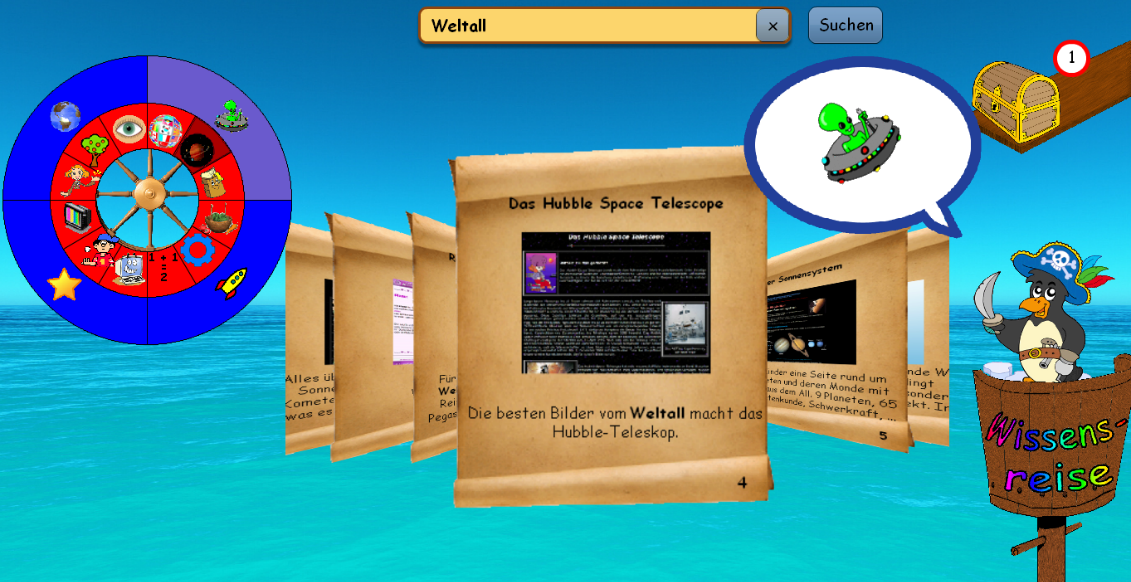
\includegraphics[width=1 \linewidth]{images/knowledge_journey.png}
    \caption{
        Screenshot of Knowledge Journey \autocite[60]{gossen2012search}
    }
    %for reference to this figure
    \label{figure:KnowledgeJourney}
\end{figure}
Their interface presents information, which can usually be retrieved with a conventional search engine, in a different way so that it is more inviting, interactable, and understandable for the minds of younger children. Furthermore, \textcite{gossen2012search} introduced a guidance character to handle possible failure and inexperience.
Another case was introduced by \textcite{alhussayen2015evaluating}, where they launched an arabic website called "Aseel Wa Raseel" that offers educational games for children. Although they used user-centered design in their development process, their platform disclosed some troubles for younger children. On their website, \textcite{alhussayen2015evaluating} included a rather long registration process, that prevented all younger children (seven to nine years old) and most of the older ones (10 to 12 years) to register on the website. 

\subsubsection{Augmented and Virtual Reality Applications}
Lastly, a rather innovative strategy is the implementation of augmented or virtual reality applications \autocite{saidin2015review, lozano2016dedigitalizing}. Based on this strategy, \textcite{kerawalla2006making}  analyzed different applications, including the solar system as the subject matter. These augmented reality applications were presented to children in elementary schools.
Although the children could create and manipulate the environment containing the planets, e.g., change size and rotation, it was mostly just animations to watch. Since the 3D animations did not require any further interaction, most children preferred simple role-play activities, where they could modify roles and interact with each other instead of only observe the 3D augmented animation \autocite{kerawalla2006making}.
Furthermore, \textcite{lozano2016dedigitalizing} introduced an educational game, that helps children build and refresh their knowledge of health literacy. With the help of tangible interfaces and mobile devices, \textcite{lozano2016dedigitalizing} succeeded to increase the motivation and satisfaction of the children. 
\textcite{saidin2015review} reviewed several different AR applications and concluded that AR has significant future potential, but still must be further developed. Most AR interfaces received positive feedback from the teacher side as well as from the student side. Especially the students proved to be more engaged with the learning process in schools \autocite{saidin2015review}.

\subsection{Why Children need different interfaces}
\label{subsection:ChildrenInterfaces}



\section{Practical Part}
\label{section:PracticalPart}
In the matter of this thesis, a study has been conducted to solidify all the findings in regards to interface design specifically made for children \autocite{gossen2012search, engen2014ipads, lozano2016dedigitalizing}. 
\\...\\

\subsection{Implementing the prototype}
\label{subsection:ImplementingPrototype}
For the implementation of this thesis, a React\footnote{https://reactjs.org/} project has been developed. As previous research from \textcite{gossen2012search, lozano2016dedigitalizing} showed, gamified approaches turned out to be more preferred by primary school children.
\\...\\

\subsection{Testing}
\label{subsection:Testing}

\begin{figure}[!ht]
    \centering
    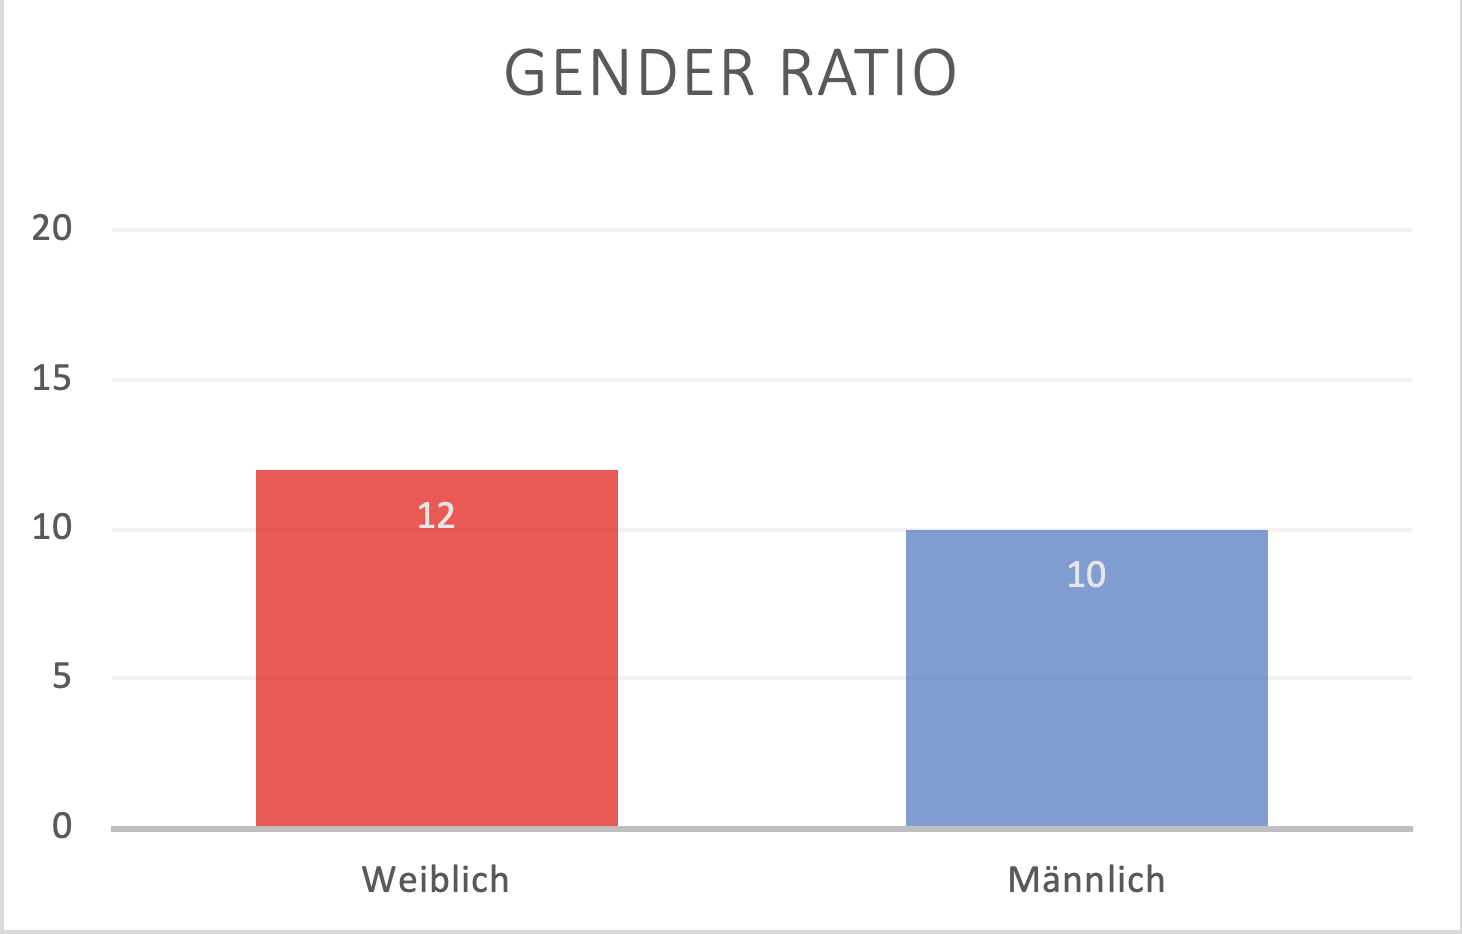
\includegraphics[width=1 \linewidth]{images/gender_ratio.png}
    \caption{
        Gender distribution between all children
    }
    %for reference to this figure
    \label{figure:GenderRatio}
\end{figure}

\begin{figure}[!ht]
    \centering
    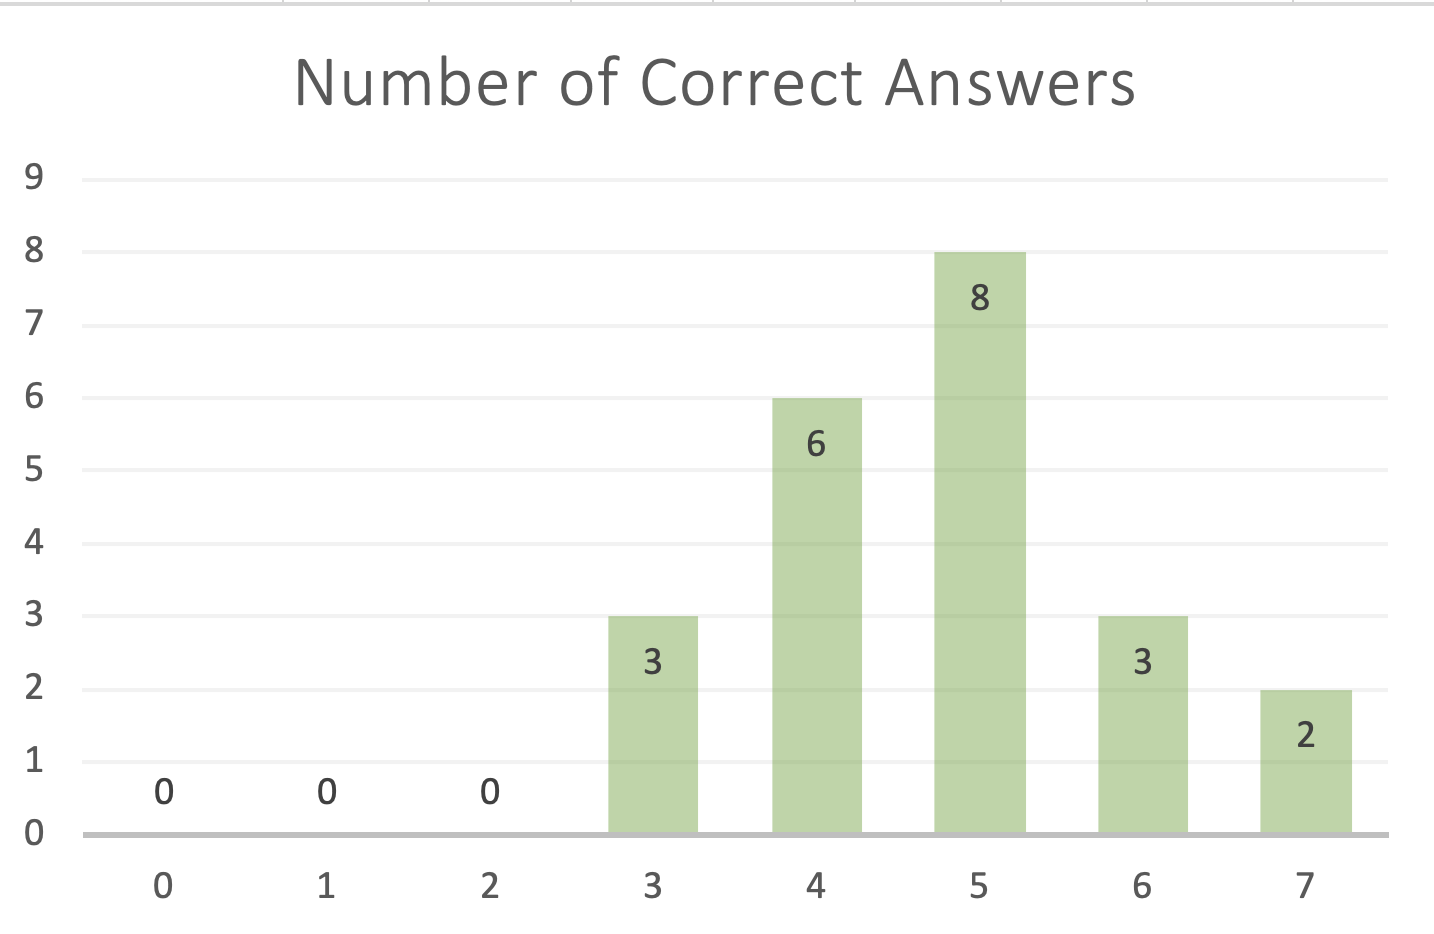
\includegraphics[width=1 \linewidth]{images/num_corr_answers.png}
    \caption{
        Distribution of correct given answers by all children
    }
    %for reference to this figure
    \label{figure:NummCorrAnswers}
\end{figure}

\subsection{Analyzing and evaluating the results}
\label{subsection:AnalyingResults}




\section{Discussion}
\label{section:Discussion}




\section{Conclusion}
\label{section:Conclusion} % the main text

%\input{acknowledgements}

\ifmmtpaper

\printbibliography

\else % only use the following for thesis format

\newpage
\printbibliography

\fi


 % group open
\ifmmtpaper 
\begingroup 
    % is required because paper template messes with sizes
    \fontsize{12}{18}\selectfont        
    \setlength{\parindent}{0pt}
    \setlength{\parskip}{5pt plus 2pt minus 1pt}
    \sectionfont{\fontsize{14}{15}\selectfont}
\fi

\newpage
\onecolumn
\begin{appendices}

%\renewcommand{\thesubsection}{\Alph{subsection}}

\section{Git-Repository}

Link zum Repository auf {\url{github.com}}:

\url{https://github.com/isperr/Bachelorarbeit_2_Sperr}


\section{Archived websites}
%\show\UrlBreaks
\sloppy
\url{http://web.archive.org/web/20190804175024/https://de.coca-cola.ch/stories/coca-cola-und-zucker}, last accessed August 12, 2019

\url{http://web.archive.org/web/20190804175135/https://www.junior.de/tipp/gesundheitsquiz/gesundheitsquiz_zaehne.php}, last accessed August 12, 2019
 
\url{http://web.archive.org/web/20180903104009/http://www.junior.de/tipp/gesundheitsquiz/vitamine.php}, last accessed August 12, 2019

\url{http://web.archive.org/web/20190804181017/https://www.kindernetz.de/infonetz/ernaehrung/ernaehrung/ernaehrungsquiz/-/id=29358/nid=29358/did=29408/1nqrl4g/index.html}, last accessed August 12, 2019

\url{http://web.archive.org/web/20190812211739/https://www.who.int/healthpromotion/conferences/9gchp/health-literacy/en/}, last accessed August 12, 2019

\end{appendices}


% group closing
\ifmmtpaper
\endgroup
\fi


\end{document}
